% CoRL 2026 workshop "Do Robots Need World Models?": CoRL template, 4 pages excluding references
% and appendices, double-blind. The submission option anonymizes the author block automatically.
% All numbers come from ../analysis.py (tab_main.tex, tab_calib.tex, tab_diff.tex, work/numbers.json).
\documentclass{article}
\usepackage{corl_2026}
\usepackage{amsmath,amssymb,booktabs,graphicx}

\title{Pixels Without Geometry? Auditing the 3D Consistency of Video World Models with Structure-from-Motion}

\author{
  Hamza Naeem\\
  \texttt{hamzanaeem588@gmail.com}
}

\begin{document}
\maketitle

\begin{abstract}
Geometric scores such as SfM registration or reprojection error are increasingly used to judge
whether video models can serve as robot world models. We show that these scores cannot be read
without motion-aware controls. On real DROID wrist-camera clips, three image-to-video models
(LTX-Video, CogVideoX, Wan2.2) and an action-conditioned DROID world model (Ctrl-World) predict the
next five seconds. We score the predictions with COLMAP, epipolar geometry and VGGT, and calibrate
each score against perturbed real continuations: non-rigid warps, approximately motion-matched
slow-downs, sharpness-matched blur and unrelated frames. The controls change the reading of the
results. Two models score \emph{better} than real footage on match counts and VGGT depth
disagreement because their predicted views barely move. LTX is worse than real footage slowed to a
similar image motion. Ctrl-World is the only model whose image motion approaches the real level,
and on these 25 clips its VGGT depth disagreement shows no statistically detectable difference from
real footage. Its features, however, do not persist across frames, and none of the models'
VGGT-estimated camera paths is reliably closer to the reference than an unrelated clip's path.
\end{abstract}

\keywords{World models, video prediction, structure-from-motion, evaluation}

\section{Introduction}
Whether robots need world models is usually argued through downstream task success. A prior
question is whether a learned model's predicted future of the robot's camera is \emph{geometrically
consistent}: one rigid scene, seen by a camera that moves as the robot moves. Structure-from-motion
(SfM) and feed-forward reconstruction offer an operational test, and they are increasingly used to
score generated video. Raw geometric scores are easy to misread, however. A frozen camera yields
clean matches and low errors without informing about 3D structure, blur removes features without
changing geometry, and non-rigid distortion can still register.

We therefore calibrate every score against controls built from the real continuation, and evaluate
general image-to-video models and an action-conditioned robot world model on real DROID wrist-camera
clips. Contributions: (i) a calibration ladder of perturbed real continuations (non-rigid warps,
approximately motion-matched slow-downs, sharpness-matched blur, unrelated frames) that shows what
COLMAP, epipolar and VGGT scores respond to; (ii) an audit with paired confidence intervals, which
shows that motion-unaware scores would rank nearly static predictions above real footage; and (iii)
a finding on the action-conditioned Ctrl-World model. Its image motion approaches the real level and
its VGGT depth disagreement shows no detectable difference from real footage, while its local
features remain temporally unstable.

\section{Related Work}
Classical geometry has been applied to generated video before: Li et al.~\citep{li2024sora} measured
SIFT/RANSAC epipolar consistency and COLMAP reconstructions on a handful of Sora, Gen-2 and Pika
clips, and MEt3R~\citep{asim2025met3r}, WorldScore~\citep{duan2025worldscore} and
GeoT2V-Bench~\citep{fan2026geot2v} score 3D consistency with feed-forward
reconstructors~\citep{wang2024dust3r,leroy2024mast3r,wang2025vggt}. Camera-controllable
generators~\citep{he2024cameractrl,xu2024camco,bahmani2025ac3d} report pose error and COLMAP success
rates, and broader benchmarks probe visual and physical
plausibility~\citep{huang2024vbench,li2025worldmodelbench,motamed2025physicsiq}. These scores are not
calibrated against perturbed real footage. For robots, video models serve as simulators and
planners~\citep{yang2024unisim,du2023unipi,ko2024avdc,zhu2025irasim,nvidia2025cosmos,jang2025dreamgen},
and action-conditioned models trained on real data, such as Ctrl-World~\citep{guo2026ctrlworld} on
DROID~\citep{khazatsky2024droid}, target policy evaluation in imagination. Robot world models are
mostly evaluated by policy-ranking agreement or visual
fidelity~\citep{quevedo2025worldgym,li2025worldeval,yue2025ewmbench}. Closest to us,
RoboPhys-3D~\citep{wang2026robophys3d} reconstructs generated robot videos with VGGT, COLMAP and SLAM,
but in simulation and without perturbed real references. We do not claim the first SfM analysis of
generated video. We contribute the calibration ladder and an audit on real robot data.

\section{Method}
\textbf{Clips and models.} From the DROID-100 sample~\citep{khazatsky2024droid} (320$\times$180, 15\,fps)
we take, per episode, the 5\,s wrist-camera window with the most image motion. A fixed mask removes
the gripper, which never moves in the wrist view. LTX-Video~\citep{hacohen2024ltxvideo},
CogVideoX-5B~\citep{yang2025cogvideox} and Wan2.2-5B~\citep{wan2025wan} receive the first frame and the
episode instruction. Ctrl-World~\citep{guo2026ctrlworld} receives the first frame of all three DROID
cameras and the \emph{recorded} end-effector poses. It rolls out at 5\,Hz in overlapping five-frame
chunks, each advancing four frames (0.8\,s). Ctrl-World thus differs from the other models in its
inputs, architecture and training data, not only in action conditioning. Outputs are resampled to
320$\times$180 and share the real first frame. All results use the 25 clips that every condition
covers. Compute (one 16\,GB laptop GPU) limited the slowest model, Wan2.2, to 25 clips
(Appendix~\ref{app:details}).

\textbf{Controls.} All controls derive from the real continuation and share the generators' H.264
round trip: \emph{real}; \emph{warp-$a$}, an independent smooth non-rigid warp per frame
($a\in\{1,2,4,8\}$\,px); \emph{slowed}, the first 40\% stretched over 5\,s, which approximately
matches LTX's average image motion at the dataset level; \emph{blurred}, Gaussian blur matched to the
sharpness of the softest outputs; and \emph{unrelated}, frames from other clips.

\textbf{Metrics.} All metrics use the 5\,s horizon at 5\,fps (every third frame, so Ctrl-World's 5\,Hz
output has no repeated frames) and frame pairs 0.4\,s apart. We use COLMAP~\citep{schonberger2016sfm}
registration rate and SIFT~\citep{lowe2004sift} + MAGSAC~\citep{barath2019magsac} epipolar inliers,
Sampson error and match-failure rate. Pairs with too few matches count as failures, and Sampson
error averages only pairs where matching and fundamental-matrix estimation succeed. Median feature
displacement serves as an \emph{image-motion proxy}. It reflects camera motion, but also scene depth,
moving objects and which features survive matching. VGGT~\citep{wang2025vggt} depth disagreement is the
median relative difference when frame $i$'s confident depth is reprojected into frame $j$. It
measures the internal consistency of VGGT's own depth and pose predictions, not ground-truth
geometry. We therefore report the fraction of points that land in frame (coverage) and a
visibility-filtered variant: confident target depth only, with points more than 10\% behind the
target surface treated as occluded. Camera-path error is the Sim(3)-aligned RMSE between the VGGT
camera centers of the prediction and of the real clip, divided by the reference path length. It
measures agreement with a \emph{VGGT-estimated reference trajectory} up to scale, not metric
ground-truth accuracy. Model-minus-control differences use paired bootstrap 95\% CIs (10,000
resamples).

\section{Results}
\begin{table}[t]
\centering
\scriptsize
\setlength{\tabcolsep}{3pt}
\resizebox{\linewidth}{!}{\begin{tabular}{lcccccccc}
\toprule
 & Motion & Reg. & Fail & Inliers & Sampson & VGGT & Cov. & Path \\
\midrule
Real & 24.2 $\pm$ 1.6 & 0.59 $\pm$ 0.08 & 0.11 $\pm$ 0.04 & 53.7 $\pm$ 8.5 & 0.32 $\pm$ 0.02 & 0.028 $\pm$ 0.003 & 0.87 $\pm$ 0.01 & 0.017 $\pm$ 0.001 \\
Slowed 2.5$\times$ & 10.9 $\pm$ 0.9 & 0.66 $\pm$ 0.07 & 0.060 $\pm$ 0.041 & 83.8 $\pm$ 11.2 & 0.26 $\pm$ 0.02 & 0.013 $\pm$ 0.001 & 0.92 $\pm$ 0.01 & 0.11 $\pm$ 0.01 \\
Blurred & 23.7 $\pm$ 1.5 & 0.76 $\pm$ 0.07 & 0.15 $\pm$ 0.04 & 57.4 $\pm$ 9.6 & 0.30 $\pm$ 0.02 & 0.029 $\pm$ 0.003 & 0.87 $\pm$ 0.01 & 0.028 $\pm$ 0.003 \\
Warp 8\,px & 24.6 $\pm$ 1.3 & 0.70 $\pm$ 0.07 & 0.15 $\pm$ 0.04 & 43.0 $\pm$ 6.4 & 0.49 $\pm$ 0.03 & 0.045 $\pm$ 0.005 & 0.85 $\pm$ 0.01 & 0.047 $\pm$ 0.004 \\
Unrelated & 118.3 $\pm$ 6.4 & 0.000 $\pm$ 0.000 & 0.84 $\pm$ 0.02 & 14.8 $\pm$ 0.8 & 0.24 $\pm$ 0.10 & 0.67 $\pm$ 0.08 & 0.18 $\pm$ 0.01 & 0.17 $\pm$ 0.01 \\
\midrule
LTX & 10.3 $\pm$ 2.0 & 0.25 $\pm$ 0.06 & 0.32 $\pm$ 0.07 & 38.8 $\pm$ 6.1 & 0.24 $\pm$ 0.03 & 0.024 $\pm$ 0.005 & 0.92 $\pm$ 0.02 & 0.15 $\pm$ 0.01 \\
CogVideoX & 2.40 $\pm$ 0.46 & 0.20 $\pm$ 0.05 & 0.023 $\pm$ 0.020 & 132.7 $\pm$ 22.3 & 0.14 $\pm$ 0.01 & 0.007 $\pm$ 0.001 & 0.98 $\pm$ 0.01 & 0.12 $\pm$ 0.01 \\
Wan2.2 & 2.57 $\pm$ 0.64 & 0.27 $\pm$ 0.07 & 0.043 $\pm$ 0.028 & 122.7 $\pm$ 17.6 & 0.16 $\pm$ 0.02 & 0.011 $\pm$ 0.002 & 0.99 $\pm$ 0.00 & 0.13 $\pm$ 0.01 \\
Ctrl-World & 19.7 $\pm$ 2.1 & 0.26 $\pm$ 0.06 & 0.36 $\pm$ 0.06 & 24.4 $\pm$ 2.0 & 0.35 $\pm$ 0.02 & 0.031 $\pm$ 0.003 & 0.86 $\pm$ 0.02 & 0.10 $\pm$ 0.01 \\
\bottomrule
\end{tabular}}
\vspace{4pt}
\caption{5\,s horizon, 25 clips common to all conditions, mean $\pm$ s.e.m. Motion: image-motion proxy
(px). Reg.: COLMAP registration rate. Fail: share of 0.4\,s frame pairs that fail to match. Sampson
in px. VGGT: depth disagreement. Cov.: fraction of reprojected points in frame. Path: camera-path
error vs.\ the VGGT-estimated reference (references: frozen camera 0.175, real path of a different
clip 0.115). Valid clips per metric are 22--25.}
\label{tab:main}
\end{table}

\begin{table}[t]
\centering
\scriptsize
\setlength{\tabcolsep}{3pt}
\begin{tabular}{lcccccc}
\toprule
 & Real & Warp-1 & Warp-2 & Warp-4 & Warp-8 & Unrelated \\
\midrule
Reprojection error (px) $\downarrow$ & 0.48 & 0.60 & 0.61 & 0.85 & 1.08 & -- \\
Median Sampson error (px) $\downarrow$ & 0.32 & 0.33 & 0.35 & 0.39 & 0.49 & 0.24 \\
Epipolar inliers per pair $\uparrow$ & 53.7 & 54.6 & 55.1 & 50.3 & 43.0 & 14.8 \\
Pairs failing to match $\downarrow$ & 0.11 & 0.11 & 0.14 & 0.10 & 0.15 & 0.84 \\
VGGT depth disagreement $\downarrow$ & 0.028 & 0.029 & 0.030 & 0.032 & 0.045 & 0.67 \\
VGGT, visibility-filtered $\downarrow$ & 0.022 & 0.022 & 0.022 & 0.024 & 0.030 & 0.20 \\
Registration rate & 0.59 & 0.73 & 0.64 & 0.56 & 0.70 & 0.000 \\
\bottomrule
\end{tabular}
\vspace{4pt}
\caption{Calibration ladder at the main settings (5\,fps, 0.4\,s pairs, same 25 clips). ``--'': too few
frames register.}
\label{tab:calib}
\end{table}

\textbf{What the scores respond to.} On the warp ladder (Table~\ref{tab:calib}), reprojection error,
Sampson error and default VGGT disagreement rise monotonically with distortion. Filtered VGGT stays
flat up to 2\,px and then rises. Registration rate fluctuates (0.59, 0.73, 0.64, 0.56, 0.70) and does
not decrease with distortion, so it is a poor measure of distortion. Neither halving image motion
nor blurring to the softest outputs' sharpness lowers registration (66\% and 76\% vs.\ 59\%,
Table~\ref{tab:main}). Slowing lowers VGGT disagreement, because frames 0.4\,s apart are closer in
viewpoint. Comparisons therefore require motion-matched references.

\begin{table}[t]
\centering
\scriptsize
\setlength{\tabcolsep}{3pt}
\resizebox{\linewidth}{!}{\begin{tabular}{lccccc}
\toprule
 & Reg. & Fail & VGGT & VGGT (filt.) & Path \\
\midrule
LTX $-$ slowed & -0.41 [-0.54, -0.28] & 0.26 [0.10, 0.41] & 0.011 [0.003, 0.021] & 0.006 [0.002, 0.012] & 0.042 [0.027, 0.058] \\
CogVideoX $-$ real & -0.39 [-0.57, -0.20] & -0.090 [-0.14, -0.043] & -0.021 [-0.028, -0.015] & -0.016 [-0.021, -0.012] & 0.099 [0.081, 0.12] \\
Wan2.2 $-$ real & -0.32 [-0.53, -0.088] & -0.070 [-0.12, -0.023] & -0.017 [-0.023, -0.010] & -0.012 [-0.017, -0.008] & 0.12 [0.095, 0.14] \\
Ctrl-World $-$ real & -0.33 [-0.49, -0.18] & 0.24 [0.17, 0.32] & 0.003 [-0.004, 0.010] & 0.003 [-0.002, 0.007] & 0.083 [0.067, 0.10] \\
Ctrl-World $-$ blurred & -0.50 [-0.64, -0.36] & 0.21 [0.13, 0.29] & 0.002 [-0.003, 0.008] & 0.003 [-0.001, 0.007] & 0.072 [0.054, 0.090] \\
\bottomrule
\end{tabular}}
\vspace{4pt}
\caption{Paired differences (model $-$ control) on the 25 clips, mean [95\% bootstrap CI]. Each model
is compared with the control matched to its confound: slowed (image motion) for LTX, blurred
(sharpness) for Ctrl-World.}
\label{tab:diff}
\end{table}

\begin{figure}[t]
\centering
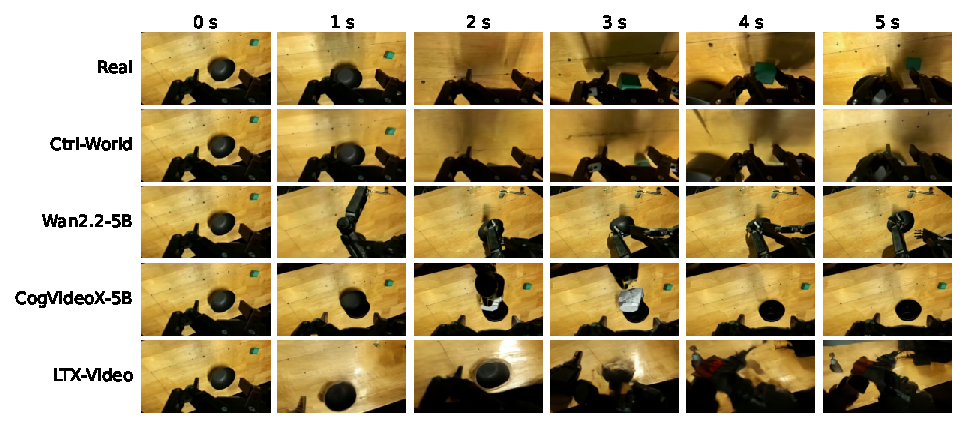
\includegraphics[width=\linewidth]{fig_qual_ep005.pdf}
\caption{One clip, 0--5\,s. Ctrl-World follows the real camera motion (softer, losing texture).
Wan2.2 cuts to a third-person view, CogVideoX holds the view while objects morph, and LTX distorts
the scene. A median-performance example is in Appendix~\ref{app:details}.}
\label{fig:qual}
\end{figure}

\textbf{Motion-unaware scores reward nearly static predictions.} CogVideoX's and Wan2.2's image motion
is about a tenth of the real level (2.4--2.6 vs.\ 24\,px). Their frames match trivially (120--130
inliers), and their match failure and VGGT disagreement are significantly \emph{lower} than real
footage's (Table~\ref{tab:diff}). Read without the motion measure, these scores would rank both models
above reality. The predicted futures are nearly static views in which objects change
(Figure~\ref{fig:qual}), and SfM registers 20--27\% of frames for lack of parallax.

\textbf{Motion-matched comparison exposes distortion.} LTX's average image motion is close to the
slowed control's (10.3 vs.\ 10.9\,px), so the two are approximately motion-matched at the dataset
level. Against that reference, LTX's registration is 41 points lower, its match failure 26 points
higher, and its VGGT disagreement higher in both variants, with all CIs excluding zero. Its low
Sampson error must be read alongside its match failures, because Sampson error summarizes only the
pairs for which geometric estimation succeeds.

\textbf{Ctrl-World: near-real motion, no detectable difference in dense consistency, unstable
features.} The action-conditioned Ctrl-World model is the only one whose image motion approaches
the real level (19.7 vs.\ 24.2\,px). On these 25 clips, its VGGT depth disagreement shows no
statistically detectable difference from real footage in either variant (+0.003, CI [$-$0.004, 0.010]
and [$-$0.002, 0.007]; real mean 0.028), at equal coverage (0.86 vs.\ 0.87). This does not establish
equivalent geometry: the intervals still allow a sizable increase. Feature-level scores disagree.
Registration is 33 points lower and match failure 24 points higher than real, and the gap is larger
still against sharpness-matched blurred real footage, so this blur setting does not explain it.
Match failures show no obvious concentration at chunk transitions (Appendix~\ref{app:details}).
The pattern is consistent with temporally unstable texture under a stable layout. Ctrl-World's
VGGT-estimated camera path is not reliably closer to the reference than an unrelated clip's real path
($-$0.015, CI [$-$0.034, 0.003]). At this resolution the path metric separates only near-exact
trajectories (re-encoded real 0.017, warps $\le$0.047). Even slowed real footage, with the right path
shape but wrong timing, does not beat the unrelated baseline.

\section{Discussion and Limitations}
Geometric scores of generated video measure several things at once: scene consistency, image motion
and feature persistence. A model that stops the camera or softens texture can look better or worse
for reasons unrelated to 3D consistency. Our calibration ladder separates these factors, and doing so
changes the conclusions. Two models that would score above real footage are nearly static, and the
action-conditioned model's low registration coexists with no detectable difference in dense VGGT
consistency. We do not claim that action conditioning causes Ctrl-World's behavior, because it also
differs in inputs, architecture and training data. Nor do we claim that these scores predict
planning success. We suggest that geometric evaluations of world models report motion-matched and
appearance-matched controls alongside raw scores. \textbf{Limitations:} one dataset and camera at low
resolution; 25 clips and small open models; DROID-100 is likely within Ctrl-World's training data (a
best case); arm and object motion violate rigidity even in real clips; image motion is a proxy for
camera motion; VGGT-based scores reflect VGGT's own predictions; and camera paths are compared to a
VGGT-estimated reference up to scale.

\bibliography{refs}

\clearpage
\appendix
\section{Implementation details}
\label{app:details}
\textbf{Generation.} LTX-Video: 704$\times$480, 121 frames at 24\,fps, 40 steps. CogVideoX-5B-I2V:
720$\times$480, 49 frames at 8\,fps, 50 steps. Wan2.2-TI2V-5B: 1280$\times$704, 121 frames at 24\,fps,
40 steps. Ctrl-World: official DROID checkpoint, replay of recorded 7-D end-effector states (xyz,
roll-pitch-yaw, gripper), 50 steps. It runs seven rollout steps at 5\,Hz, each generating five frames
that include the previous step's last frame, so each step advances four frames (0.8\,s). Of the 29
frames, the first 26 (5\,s) are kept. The 5B transformers store weights in fp8 and compute in bf16.
One prompt template uses the episode instruction (a neutral instruction where DROID-100 has none).
Clips are the 60 highest-motion windows of DROID-100. LTX and Ctrl-World cover all 60, CogVideoX 40
and Wan2.2 25. All reported results use the 25 clips common to every condition.

\textbf{Scoring.} COLMAP incremental SfM with one shared SIMPLE\_RADIAL camera, sequential matching
(overlap 10), SIFT at doubled resolution, and initialization and registration thresholds lowered to
40 and 15 inliers for 320$\times$180 frames. Epipolar pairs need at least 16 ratio-test matches, or
they count as match failures. VGGT runs on the 26 frames of the 5\,fps track, and source points are
those above the median depth confidence. The slowed control (2.5$\times$) approximately matches LTX's
average image motion. The blur ($\sigma=0.7$\,px) matches the Laplacian-variance sharpness of
Ctrl-World and LTX. The path-error reference ``unrelated clip'' averages each clip's error against
the real paths of all 24 other clips. The frozen-camera reference collapses all predicted centers to
one point.

\textbf{Chunk transitions.} On the 5\,fps track, the share of consecutive Ctrl-World frame pairs that
fail to match is 16\%, 20\%, 21\% and 23\% at the four positions within a rollout step (the last
position crosses into the next step), against 3--5\% for real footage. We see no obvious
concentration at the transition, although this coarse test cannot rule out subtler boundary effects.

\textbf{Additional example.} Figure~\ref{fig:qual2} shows a clip near the median of both Ctrl-World's
and LTX's registration rates.

\begin{figure}[h]
\centering
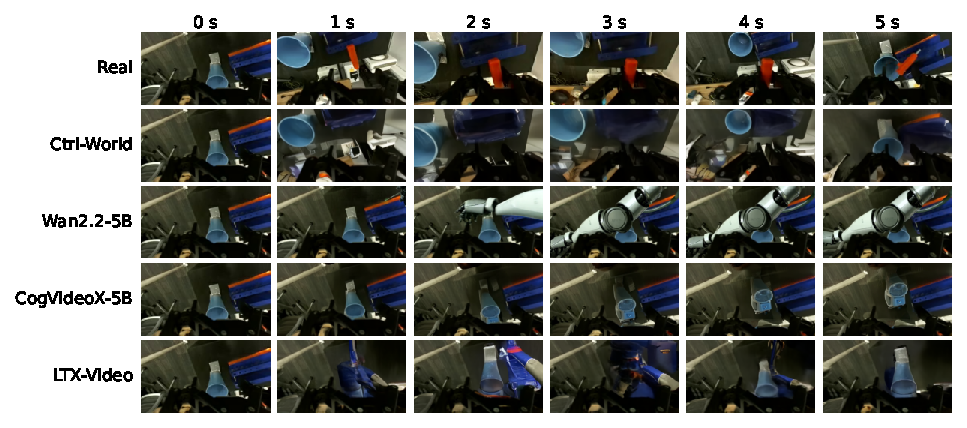
\includegraphics[width=\linewidth]{fig_qual_ep008.pdf}
\caption{A representative clip (near the median registration of Ctrl-World and LTX). Ctrl-World
follows the real camera's sweep. Wan2.2 and CogVideoX hold the viewpoint while objects change, and
LTX distorts the scene.}
\label{fig:qual2}
\end{figure}

\textbf{Code.} All code will be released after review.

\end{document}
